% Ejemplo de documento LaTeX
% Tipo de documento y tamaño de letra
\documentclass[10pt]{article}
% Preparando para documento en Español.
% Para documento en Inglés no hay que hacer esto.
\usepackage[spanish]{babel}
\selectlanguage{spanish}
\usepackage[utf8]{inputenc}


% EL titulo, autor y fecha del documento
\title{Tiro parabólico con fricción del aire}
\author{Rios Quijada Danira}
\date{10 de Abril de 2015}
% Aqui comienza el cuerpo del documento
\usepackage{graphicx}
\begin{document}
% Construye el título
\maketitle
\section{Introducción}
En esta práctica, realizamos un programa en FORTRAN para calcular la posición de un objeto lazado con tiro parabólico, en ciertos instantes de tiempo, tanto en condiciones ideales, como tomando en concideracion la resistencia del aire y comparando ambos resultados.
\\
\\
\\
\section{Un poco de física}
En nuestro estudio del movimiento de proyectiles, habitualmente despreciamos la resistencia del aire, sin embargo esta tiene un efecto apreciable en el movimiento de proyectiles.\\

No es dificil incluir la resistencia del aire en las ecuacuaciones del proyectil, pero resolverlas para la posicion y la velocidad en funcion del tiempo puede resultar un poco complejo.\\

Cuando omitimos la resistencia del aire, la unica fuerza actuando en el proyectil es el peso $p=mg$ y los componentes de la aceleracion son sencillos $a_{x}=0$ y $a_{y}=-g$.\\

Ahora incluyendo la resistencia del aire actuando sobre el proyectil,la $f$ sera mas o menos proporcional  al cuadrado de la velocidad del proyectil. $f=Dv^2$, donde $v^2=v_{x}^2+v_{y}^2$. La direccion de $f$ es opuesta a la direccion de $v$ por ende $f=-Dvv$. Entonces: $f_{x}=-Dvv_{x}$ y $f_{y}=-Dvv_{y}$.\\

Por la segunda ley de Newton $a_{x}=-(D/m)vv_{x}$ y $a_{y}=-g-(D/m)vv_{y}$.\\

La constante D depende de la densidad del aire, asi como del area en contacto del proyectil y el coeficiente de friccion del tipo de proyectil.$D=(\rho(CA))/2$.\\

Los componentes de la aceleracion estan en constante cambio al igual que los componentes de la velocidad, pero en periodos de tiempo pequeños $\Delta(t)$.Durante el intervalo de tiempo $\Delta(t)$ $a_{x}=\Delta(v_{x})/(\Delta(t))$ y la velocidad en x cambiar de acuerdo a $\Delta(v_{x})=a_{x}\Delta(t)$, lo mismo pasa con los componentes en y. Llegamos a  $v_{x}+\Delta(v_{x})=v_{x}+a_{x}\Delta(t)$ y $v_{y}+\Delta(v_{y})=v_{y}+a_{y}\Delta(t)$.\\

Mientras el proyectil se mueve sus coordenadas logicamente estan cambiando, la coordenada x cambia de la siguiente manera: $\Delta(x)=(v_{x}+\Delta(v_{x})/2)\Delta(t)=v_{x}\Delta(t)+1/2a_{x}(\Delta(t))^2$ en el eje y es exactamente la misma expresion. Entonces las coordenadas del proyectil para el final del intervalo son: \\

$x+\Delta(x)=x+v_{x}\Delta(t)+1/2a_{x}(\Delta(t))^2$ y $y+\Delta(y)=y+v_{y}\Delta(t)+1/2a_{y}(\Delta(t))^2$\\ 

\section{Código}

El código que utilizamos para realizar el programa fue el siguiente:\\
\begin{verbatim}  
 !Con este programa podremos calcular la posicion de un proyectil en tiro parabolico, conciderando la resistencia del aire y comparalo con una situacion ideal.

program tiro_resistencia

implicit none
real, parameter :: deltat = 0.01
real, parameter :: g = 9.81 !Valor de la gravedad
real, parameter :: pi=4.0*ATAN(1.0)
real, parameter :: densidad = 1.18 !Densidad del aire al nivel del mar
real, parameter :: cfe = 0.47

integer, parameter :: npts= 2000 

real :: xi, yi, vi, theta, radianes
real :: xmaxsf, ymaxsf, timesf, xmaxcf, ymaxcf, timecf
real :: diferenciax
write (*,*), 'Deme las coordenadas iniciales de x en m'
read *, xi
write (*,*), 'Deme las coordenadas iniciales de y en m'
read *, yi
write (*,*), 'Deme la velocidad inicial del proyectil en m/s'
read *, vi
write (*,*), 'Deme el angulo inicial de tiro en grados'
read *, theta

radianes = (theta*pi)/180.0

call sin_friccion (xi,yi,vi,radianes,xmaxsf,ymaxsf,timesf)
call con_friccion (xi,yi,vi,radianes,xmaxcf,ymaxcf,timecf)


diferenciax = 100.0-((xmaxcf*100.0)/xmaxsf)



print *, "#####################################################"
print *, "||En condiciones ideales||"
print *, "Un tiro parabolico con:"
print *, "coordenadas iniciales x=",xi,"y=",yi
print *, "velocidad inicial", vi,"m/s"
print *, "y un angulo de", theta, "grados"
print *, "durara en el aire un tiempo de:", timesf,"s"
print *, "alcanzara una h maxima de:", ymaxsf,"m"
print *, "tendra un alcanze maximo en el eje x de:", xmaxsf,"m"
print *, "#####################################################"
print *, "||Con resistencia del aire||"
print *, "Un tiro parabolico con:"
print *, "coordenadas iniciales x=",xi,"y=",yi
print *, "velocidad inicial", vi,"m/s"
print *, "y un angulo de", theta,"grados"
print *, "durara en el aire un tiempo de:", timecf,"s"
print *, "alcanzara una h maxima de:", ymaxcf,"m"
print *, "tendra un alcanze maximo en el eje x de", xmaxcf,"m"
print *, "#####################################################"
print *, "La diferencia porcentual en el eje x es:", diferenciax,"%"
print *, "#####################################################"


end program tiro_resistencia


subroutine sin_friccion (xi,yi,vi,radianes,xmaxsf,ymaxsf,timesf)

implicit none
real, parameter :: deltat = 0.01
real, parameter :: g = 9.81 !Valor de la gravedad
real, parameter :: pi=4.0*ATAN(1.0)
real, parameter :: densidad = 1.18 !Densidad del aire al nivel del mar
real, parameter :: cfe = 0.47

integer, parameter :: npts= 2000 

real, dimension (1:npts) :: x,y,t
real :: xi, yi, vi, radianes !Entran
real :: xmaxsf, ymaxsf, timesf !Devuelve

integer :: i


xmaxsf = xi+((vi*vi*sin(2*radianes))/(g))
ymaxsf = yi+(((vi*vi)*(sin(radianes)*sin(radianes)))/(2*g))
timesf = (2*vi*sin(radianes))/(g)

!Registramos los datos calculados
open (1, file="sin_friccion.dat")

!Calculando la posicion para cada t(i)
do i=1, npts
t(i)=float(i)*deltat
x(i) = xi + (vi*cos(radianes)*t(i))
y(i) = yi + (vi*sin(radianes)*t(i)) - ((0.5*g)*t(i)*t(i))

!Registrando resultados
write (1,*) x(i), y(i)
if (y(i)<0) exit
end do

CLOSE (1)
end subroutine sin_friccion

!#####################################################################

subroutine con_friccion (xi,yi,vi,radianes,xmaxcf,ymaxcf,timecf)

implicit none

real, parameter :: deltat = 0.01
real, parameter :: g = 9.81 !Valor de la gravedad
real, parameter :: pi=4.0*ATAN(1.0)
real, parameter :: densidad = 1.18 !Densidad del aire al nivel del mar
real, parameter :: cfe = 0.47

integer :: i 

integer, parameter :: npts= 2000 

real, dimension (0:npts) :: xx,yy,tt,velxx,velyy,axx,ayy 
real :: xi, yi, vi, radianes !Entrada
real :: xmaxcf, ymaxcf, timecf !Salida
real :: D, area, radio,masa !D representa una constate que depende del area, 
!el coeficiente y la densidad

print *, "Deme la masa de la esfera en kg"
read *, masa


print *, "Deme el radio de la esfera en m"
read *, radio

area = pi*radio*radio



!Definiendo condiciones iniciales
xx(0) = xi
yy(0) = yi

velxx(0) = vi*cos(radianes)
velyy(0) = vi*sin(radianes)

D = (0.5*densidad*area*cfe)

axx(0) = -(D/masa)*(sqrt((velxx(0)*velxx(0))+(velyy(0)*velyy(0))))*velxx(0)
ayy(0) = -g-(D/masa)*(sqrt((velxx(0)*velxx(0))+(velyy(0)*velyy(0))))*velyy(0)

tt(0) = 0
!Abriendo archivo.dat 
open (2, file="con_friccion.dat")

!Registrando valores iniciales
write(2,*) xx(0),yy(0)



!Calculando velocidad, aceleracion y posicion para cada t(i)
do i=0, npts

tt(i+1) = tt(i) + deltat

velxx(i+1) = velxx(i)+axx(i)*tt(i+1) 
velyy(i+1) = velyy(i)+ayy(i)*tt(i+1)

axx(i+1) = -(D/masa)*(sqrt((velxx(i)*velxx(i))+(velyy(i)+velyy(i))))*velxx(i)
ayy(i+1) = -g-(D/masa)*(sqrt((velxx(i)*velxx(i))+(velyy(i)+velyy(i))))*velyy(i)

xx(i+1) = xx(i)+velxx(i)*tt(i+1)+(0.5*axx(i)*tt(i+1)*tt(i+1))
yy(i+1) = yy(i)+velyy(i)*tt(i+1)+(0.5*ayy(i)*tt(i+1)*tt(i+1))

!Registrando valores 
write (2,*) xx(i+1), yy(i+1)
if (yy(i+1)<0) exit
end do

close (2)
xmaxcf = xx(i)!El alcanze en x 
ymaxcf = MAXVAL(yy) !EL alcanze en y
timecf = tt(i)*10.0 !El tiempo esta en s/10, por eso lo multiplicamos por 10

end subroutine con_friccion

\end{verbatim} 

\newpage
\subsection{Resultados}
Cabe denotar que en el código se cambia la salida estándar de los datos de posición a 2 archivos, llamados ``sinfriccion.dat''y ``confriccion.dat, los cuales utilizamos posteriormente para graficar las coordenadas con gnuplot.Una vez concluido el programa, lo compilamos, he aquí los resultados al ejecutarlo con los ángulos de 30, 60 y 45 grados.

\subsubsection{30 grados}
\begin{tabular}{c}
\begin{center}
   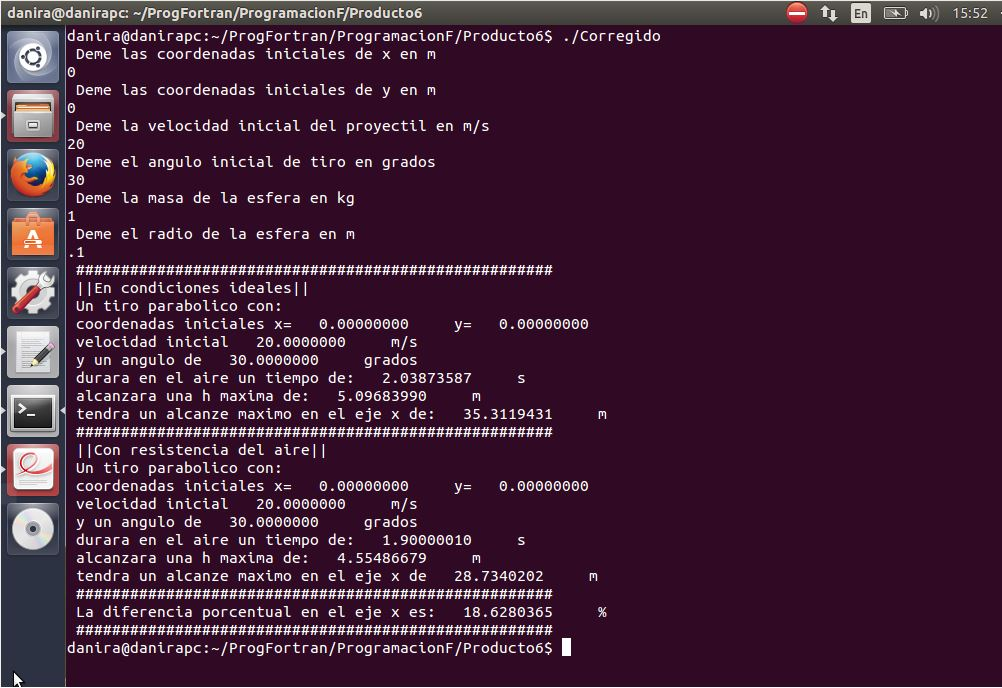
\includegraphics[scale=0.4]{30grados.JPG}
\end{center}
\end{tabular}

\subsubsection{45 grados}
\begin{tabular}{c}
\begin{center}
   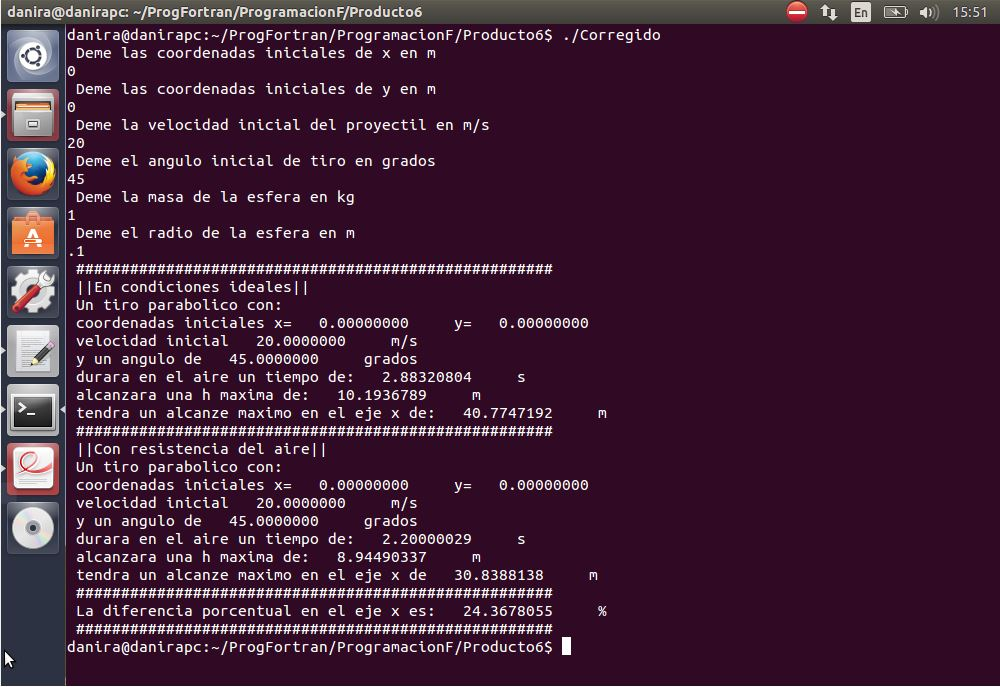
\includegraphics[scale=0.4]{45grados.JPG}
\end{center}
\end{tabular}

\subsubsection{60 grados}
\begin{tabular}{c}
\begin{center}
   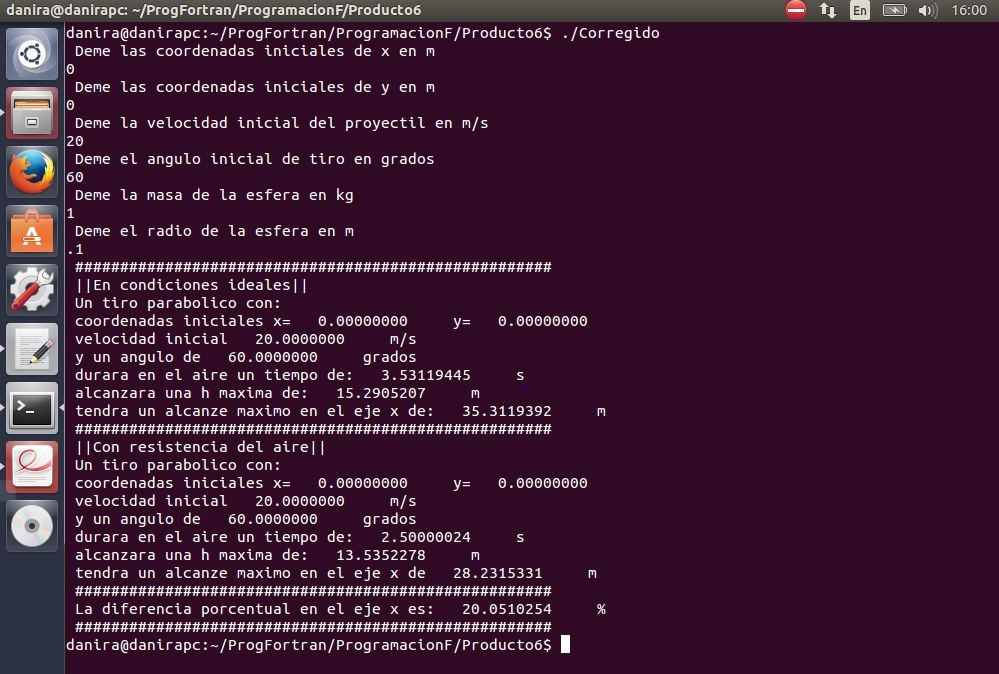
\includegraphics[scale=0.4]{60grados.JPG}
\end{center}
\end{tabular}




\newpage


\section{Graficando con Gnuplot}
En esta parte de la práctica nos enfocamos en graficar la información que se capturo en los archivos, para eso utilizamos gnuplot.
\space
Obteniendo el siguiente resultado para cada ángulo de prueba;


\subsection{30 grados sin fricción}
\begin{center}
   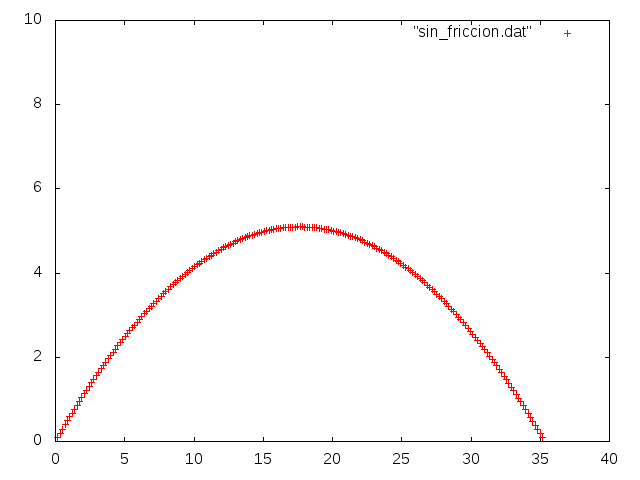
\includegraphics[scale=0.5]{30gradosnf.png}
\end{center}

\subsection{30 grados con fricción}
\begin{center}
   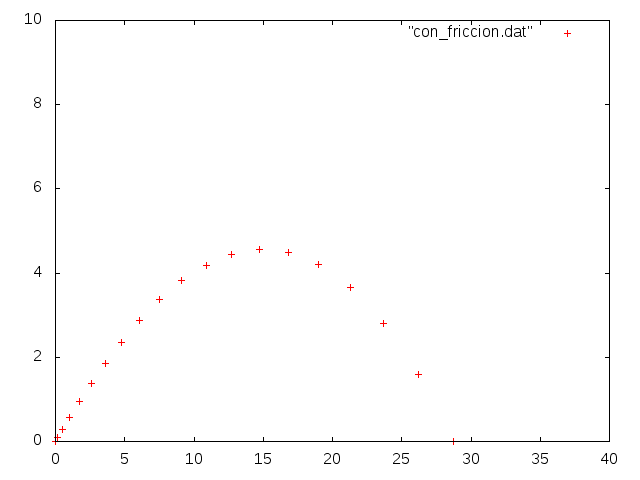
\includegraphics[scale=0.5]{30gradoscf.png}
\end{center}


\subsection{45 grados sin fricción}
\begin{center}
   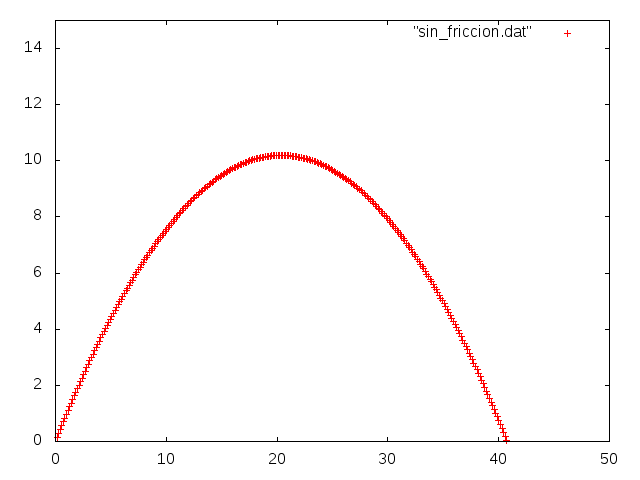
\includegraphics[scale=0.5]{45gradosnf.png}
\end{center}

\subsection{45 grados con fricción}
\begin{center}
   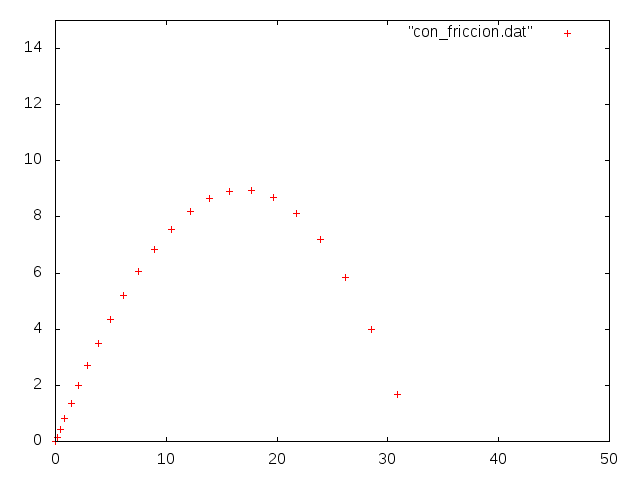
\includegraphics[scale=0.5]{45gradoscf.png}
\end{center}


\subsection{60 grados sin fricción}
\begin{center}
   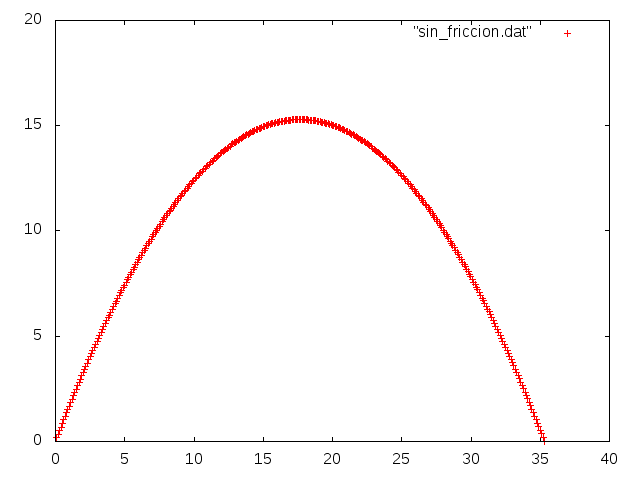
\includegraphics[scale=0.5]{60gradosnf.png}
\end{center}

\subsection{60 grados con fricción}
\begin{center}
   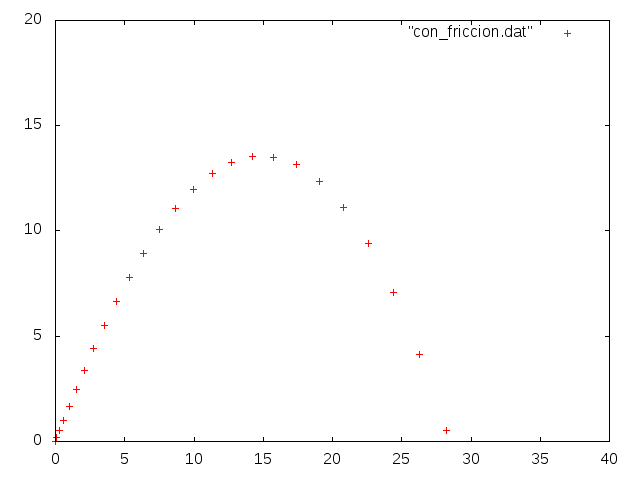
\includegraphics[scale=0.5]{60gradoscf.png}
\end{center}



% Nunca debe faltar esta última linea.
\end{document}
